\documentclass[a5paper]{article}

\usepackage{eaj}
\usepackage{float}

\title{\textb{Refleksjonsnotat} \\ {\large TPD4114 Visuell formidling}}
\author{Erik André Jakobsen}
\date{Høsten 2019}


\begin{document}
\RaggedRight

\maketitle

\section*{Filosofi for presentasjonen}
I presentasjonen ønsket jeg å ta for meg noe relatert til praktisk bruk av matematikk og/eller datavitenskap. Bakgrunnen for dette er at selv om de aller fleste er overbevist om \emph{at} disse fagområdene er viktige og interessante, er det ofte vrient å komme på enkle, konkrete grunner til nettopp hvorfor det på stående fot. Selv om tema jeg endte opp med å snakke om først fremstår trivielt, forsøker jeg i slutten å overbevise om at disse har bruksområder i den virkelige verden.

I arbeidet med dette opplevde jeg det som er et kjent dilemma for alle formidlere av kunnskap: Hvor skal vi trekke grensen mellom hva som er for komplisert, og hva som er for enkelt til å være representativt? For eksempel lærer alle som tar et kurs i fysikk Newtons berømte formel $F = ma$, som forteller oss at netto kraft som virker på et objekt er produktet av objektets masse og akselerasjon. Dette er en sjokkerende enkel formel, og den virker bra nok til å lande en rakett på månen -- men den er likevel bare en approksimasjon av virkeligheten. Det korrekte uttrykket er på formen
\begin{equation*}
    F = \frac{d}{dt} \left( \frac{m_0 v}{\sqrt{1 - \left( v/c \right)^2}} \right)
\end{equation*}
som er en del mer omfattende enn det forrige. Nøkkelen her er at nesten alt i ligningen over er uviktig støy. Så lenge objektet vi er opptatt av beveger seg mye saktere enn lysets hastighet (og det gjør jo det aller, aller meste\footnote{Såvidt jeg vet, i alle fall}). Om fysikkursene hadde dundret rett i gang med dette kompliserte uttrykket, hadde de fleste som skulle lære fysikk falt av med en gang, eller i alle fall bruke veldig lang tid på å forstå hva kraft i det hele tatt er, rent konseptuelt. Læringen går tapt i detaljene.

Tilsvarende hensyn er tatt i utformingen av denne presentasjonen. Det er mange detaljer som er hoppet glatt over: Hvordan informasjon lagres i minnet på en datamaskin, hvordan vi kan bevise at en algoritme er korrekt, hvordan vi henter ut minste tall i en samling av mange tall på mest mulig effektiv måte, og så videre. Ingen av disse detaljene er viktige i det vi holder på med nå. Det interessante er hvordan kan vi løse problemet vi står ovenfor, rent konseptuelt.

\section*{Problemet}
I prosjektet vil jeg se på hvordan en datamaskin kan løse labyrinten som denne:
\begin{figure}[H]
    \centering
    
\includegraphics{liten_labyrint_forstor.png}
\end{figure}
For oss er dette et veldig enkelt problem. I dette tilfellet finner vi løsningen bare ved å se på labyrinten. Hva gjør vi derimot om labyrinten ser ut som følgende?
\begin{figure}[H]
    \centering
    
\includegraphics[scale=0.6]{combo400.png}
\end{figure}
Da blir ting plutselig litt verre. Heldigvis finnes det måter å løse dette på ved hjelp av datamaskiner. Å gjøre dette fremstår kanskje som litt umotivert, eller i det minste litt bortkastet. Hvilken nytteverdi har det å løse labyrinter? Selv om det virker ganske fjernt, er det nøyaktig det som skjer når du bruker ditt favorittkart til å finne veien til et nytt sted:
\begin{figure}[H]
    \centering
    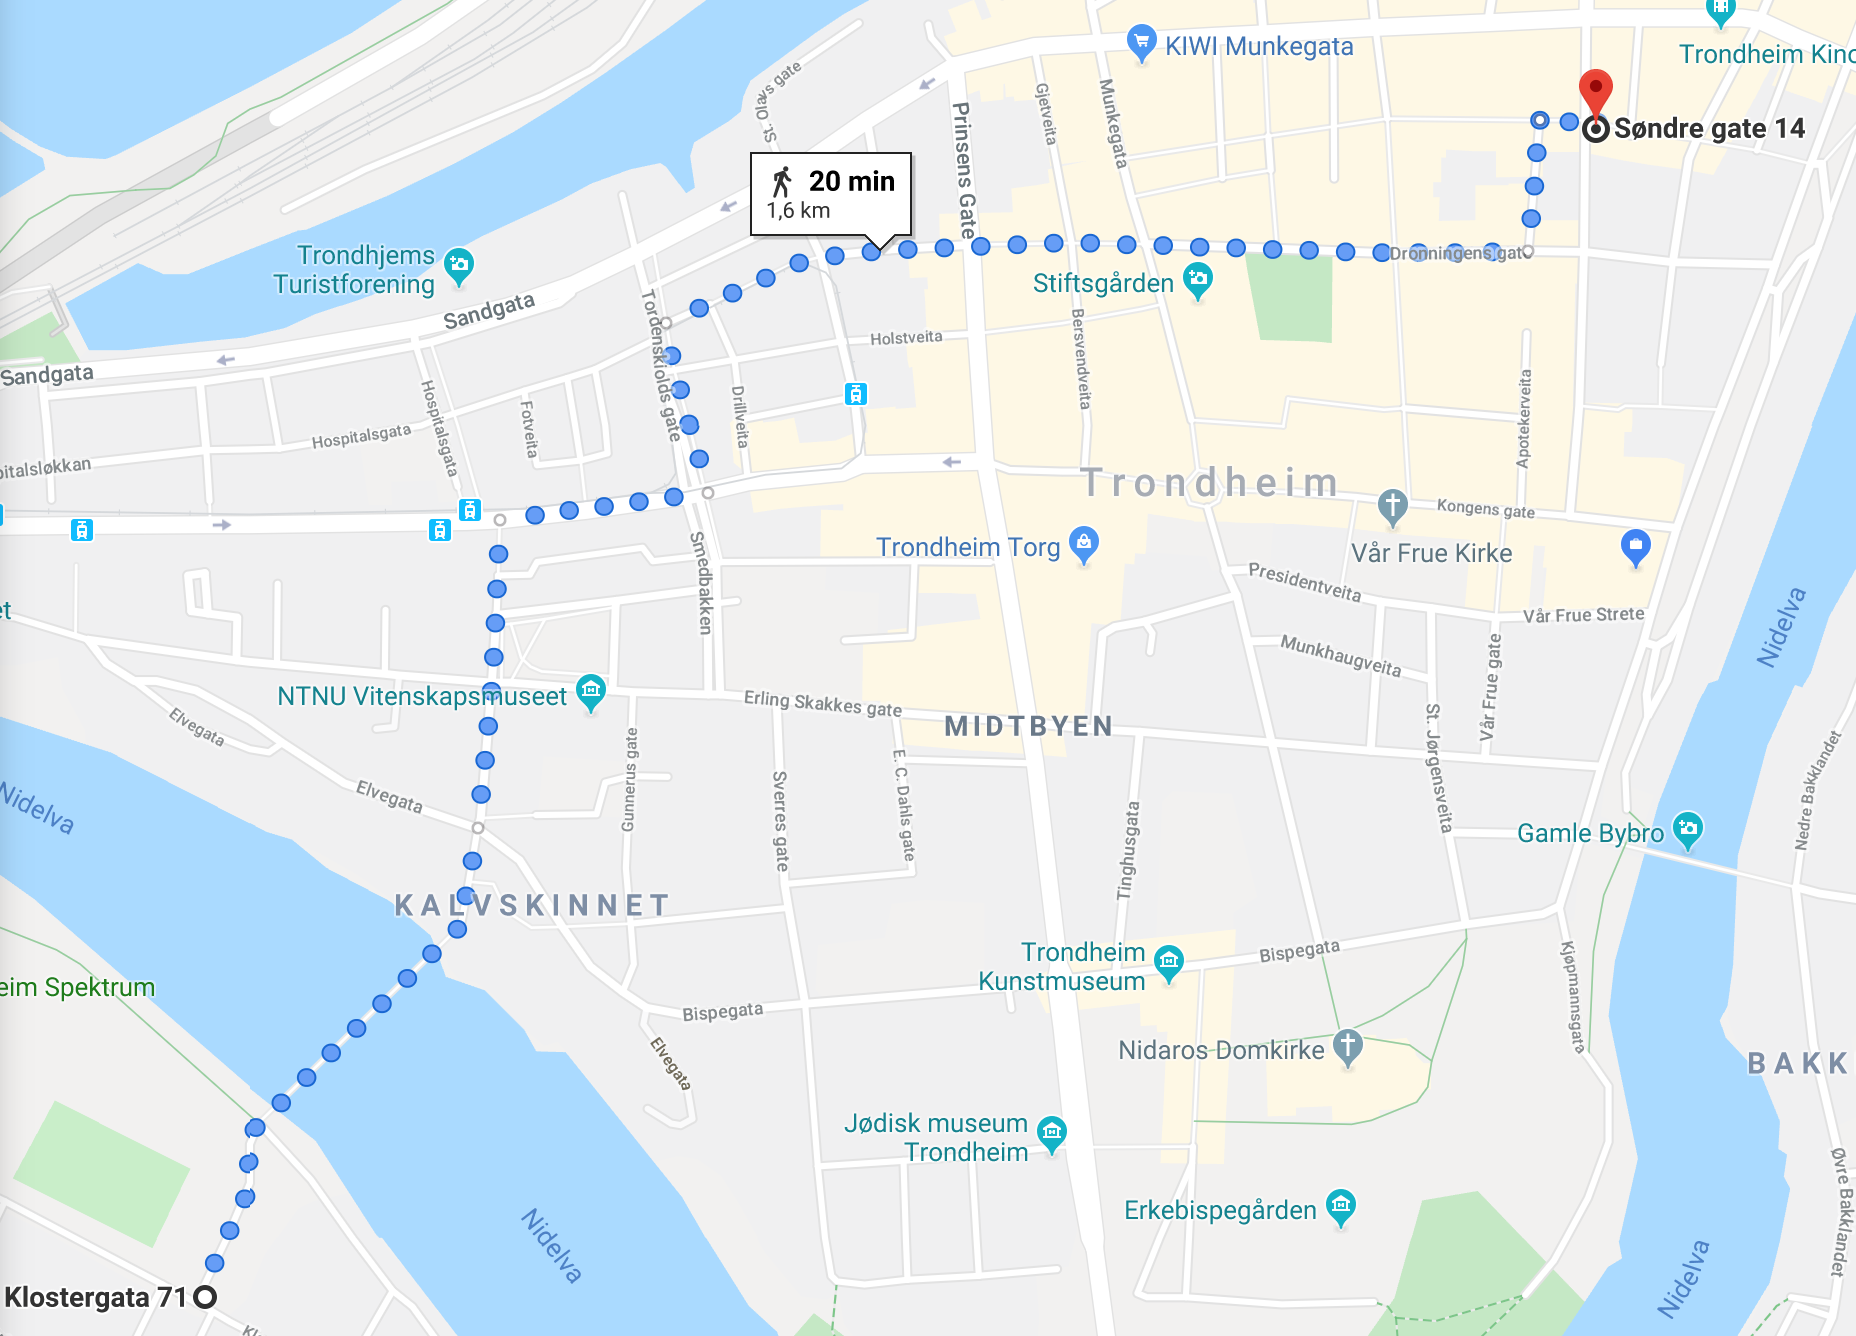
\includegraphics[width=0.8\linewidth]{google-maps.png}
\end{figure}
Den underliggende strukturen i våre enkle labyrinter er så godt som identisk med den som ligger under kart, og måten vi finner løsninger på \emph{er} identiske.

\section*{Utfordringer}
Ved starten av av prosjektet innså jeg at det var mange fremmedord i presentasjonen. Ord som algoritme, node, vektet kant, og andre begreper som nok ikke er fullstendig nye for de fleste, men som kan være fremmede nok til å gjøre betydningen mer vanskelig enn den trenger å være.
\end{document}